\section{Introduction}

A redundant manipulator can reach a Cartesian target through different joint paths and terminal poses, changing motion duration, electrical energy, and proximity to joint limits or singularities. Energy-aware robot planning has developed from torque-based surrogates \cite{r1} to electrical consumption models \cite{r2,r3,r4}. Kinematic redundancy and manipulability provide further degrees of freedom for selecting feasible motions \cite{r5,r6}. The resulting planning problem must balance time and energy while maintaining constraints that remain feasible during execution.

Execution introduces a separate challenge. Payload variation, friction mismatch, and external disturbances require feedback corrections to nominal torque commands \cite{r16,r18}. Control barrier function (CBF) quadratic programs (QPs) modify nominal inputs when necessary to enforce safety conditions \cite{r7,r8}. Hierarchical planning can coordinate reference generation and feedback control \cite{r15}. Observer-informed and robust CBF methods address uncertainty in online safety filtering \cite{r9,r10,r11,r12}, while prescribed-time manipulator safety and singularity avoidance have also been studied \cite{r13,r14}. However, online correction of a nominal command \cite{r9,r10} does not establish its feasibility under an upstream energy-optimized plan. Hard actuator limits can also conflict with barrier requirements.

The main challenge is therefore to construct a time-energy plan that accounts for the constraints of its execution filter before motion begins. Replacing a time-varying margin by its largest allowance over the motion can unnecessarily tighten the plan. Moreover, state-dependent torque and relative-degree-two barrier conditions require different uncertainty allowances. The planning margins must follow from the closed-loop error dynamics and verified bounds over the execution tube, rather than from an assumption of exact trajectory tracking.

The proposed architecture (Fig.~\ref{fig_workflow}) couples free-duration quintic B-spline planning with an online robust high-order CBF-QP. We use the established generalized momentum observer \cite{r17} and Slotine-Li tracking law \cite{r18} to obtain the disturbance and tracking-error dynamics needed to construct the proposed time-varying margins. With validated bounds and positive reserves, the QP leaves nominal tracking torque unchanged while the stated constraints hold. A braking-oriented soft-QP handles hard-QP infeasibility by retaining torque limits and requesting replanning, without asserting barrier invariance during recovery.

The main contributions are summarized as follows.
\begin{enumerate}
\item A free-duration quintic B-spline planner that minimizes a weighted sum of approximate non-regenerative electrical energy and motion duration while optimizing the redundant
terminal configuration under execution-tightened constraints.

\item Time-varying torque, velocity, and high-order barrier
margins derived from observer, tracking, and torque-residual
envelopes, yielding a feasible set no smaller than that of
their corresponding constant worst-case envelopes.

\item Conditional planner-filter consistency establishing
when the robust HOCBF-QP leaves the nominal tracking
torque unchanged while preserving joint-position,
joint-speed, torque, and manipulability limits,
complemented by torque-bounded soft-QP recovery
outside the certified regime.
\end{enumerate}

\begin{figure}[!t]
\centering
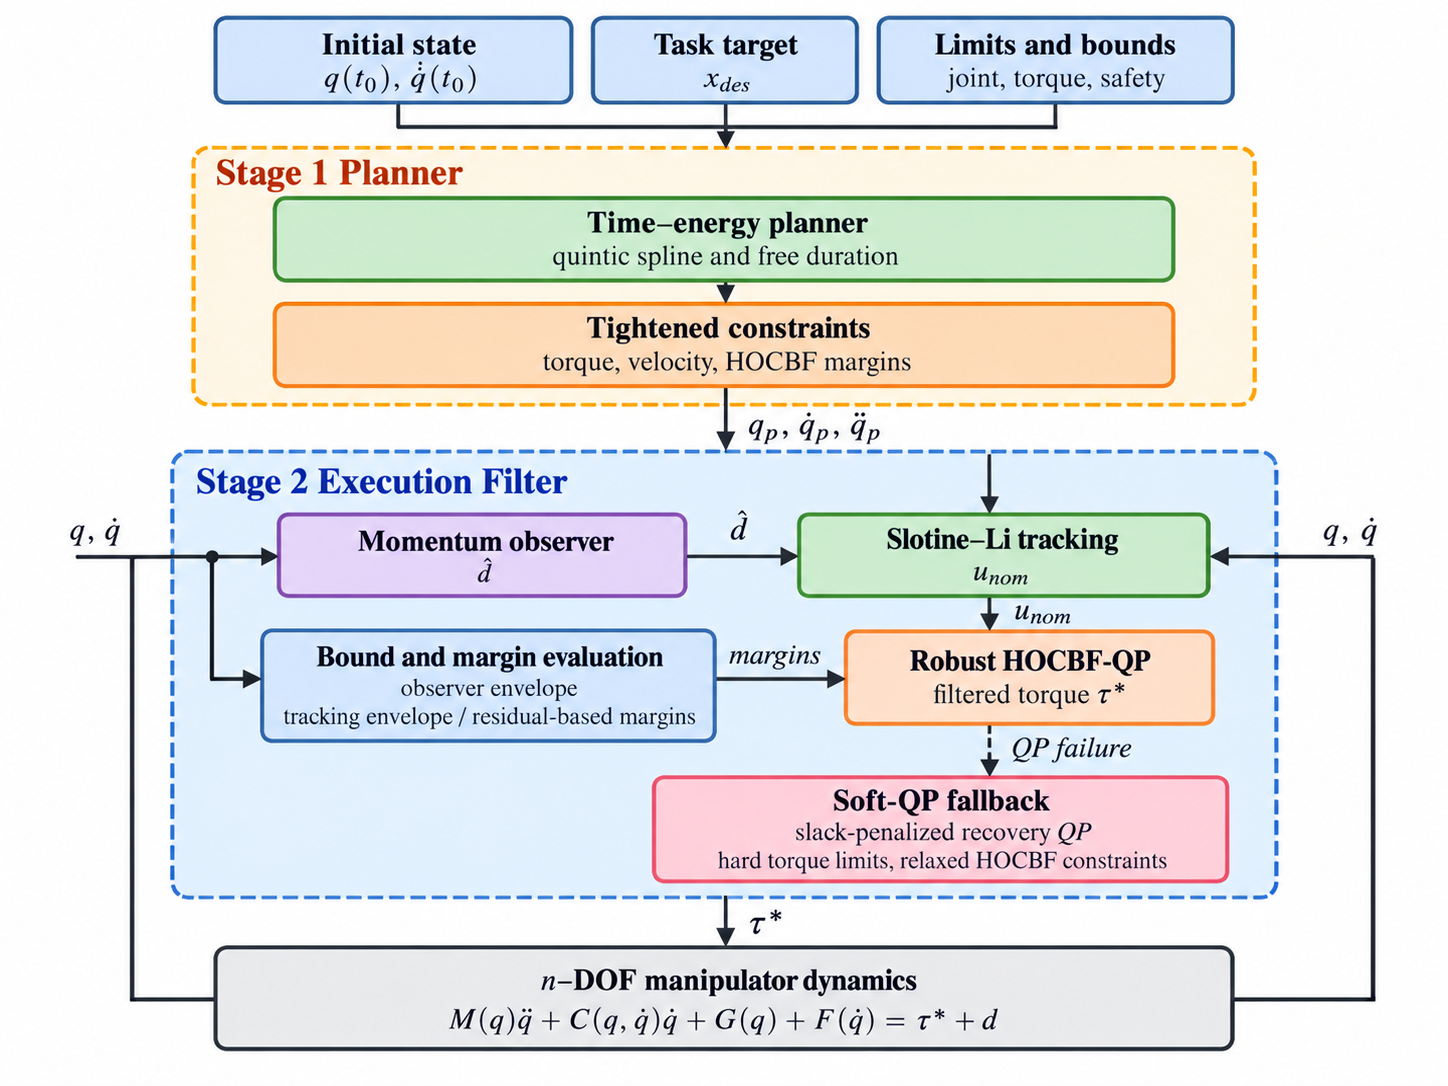
\includegraphics[width=0.98\columnwidth]{fig/fig_0.png}
\vspace{-1.6mm}
\caption{Planner-filter architecture and infeasible-QP recovery.}
\label{fig_workflow}
\vspace{-2mm}
\end{figure}
